\documentclass[reprint, english, nofootinbib]{revtex4-2}

\usepackage{graphicx}
\usepackage{subfig}
\usepackage[colorlinks=true,urlcolor=blue,citecolor=blue]{hyperref}
\usepackage{physics}
\usepackage{amsmath}
\usepackage{amssymb}
\usepackage{amsbsy}
\usepackage{subfig}
\usepackage{blindtext}
\usepackage{tikzducks}
\usepackage{tikz}
\usepackage{pgfplots}
\usepackage{listings}

\graphicspath{{../figs/}}


\begin{document}
\title{Solving Differential Equations with Neural Networks}
\author{Nicholas Karlsen}
\affiliation{University of Oslo}
\author{Thore Espedal Moe}
\affiliation{University of Oslo}
\date{\today}

\begin{abstract}
    \noindent
    We investigate the application of neural networks to the solution of both partial differential equations, exemplified by the 1-D heat equation; as well as systems of nonlinear ordinary differential equations, exemplified by a system of equations describing the dynamics of a class of Recurrent Neural Networks that can be used to find eigenvalues and eigenvectors of a real, symmetric matrix. For the heat equation we compare the solution from a neural network with both the analytic solution and a numerical solution from a simple Finite-Difference scheme for different resolutions of the computational grid and different amounts of training points for the network. We perform a similar analysis for the nonlinear system; this time comparing the networks solution with a numerical integration using the Forward-Euler method. However, as the nonlinear system does not readily admit an analytical solution, only the equilibrium state of the system can be independently computed (through standard numerical eigendecomposition of the mentioned matrix) as a "ground truth" of the solution. In general we find that the neural network-based solution can reach a reasonable level of accuracy with fewer grid-points/training points than the standard numerical integration schemes, and with far less stringent requirements on the distance between grid-points. Notably, the neural network-solution does not need its training grid-points to satisfy the famously restrictive stability criterion for the Finite-Difference method applied to the heat equation. We do find, however, that it is more difficult to scale up the accuracy of the network-based solutions, as compared to more traditional schemes.
\end{abstract}

\maketitle

\section{Introduction}
\noindent
Per the preponderating proliferation of differential equations in the sciences, both natural and otherwise, there is intense and inherent interest in novel ways of obtaining their solutions. Thus, one of the more exciting developments in machine learning, and the topic of this paper, is the application of neural networks to the task of solving differential equations. 

We will be looking at two distinct problem types; partial differential equations (PDE) and systems of nonlinear ordinary differential equations (ODE). Concretely, we will be using the 1-D heat equation as an example of a PDE, while a method from \cite{Yi_2004} for finding eigenvalues and eigenvectors of real and symmetric matrices will serve as the example of nonlinear systems of ODEs.

In both cases we will compare solutions obtained from neural network-based approaches with those from more traditional numerical methods, namely the simplest available Finite-Difference schemes. For the heat equation an analytic solution is easily obtained as the ground truth of the methods. For the eigenproblem-related system an analytic solution is not easily acquired; rather, as the steady-state equilibrium points of the system correspond to the eigenvectors of a given matrix, the asymptotic solution can be computed by standard numerical eigendecomposition of the matrix.

Structurally, we begin with a brief discussion of how neural networks can be applied to solve differential equations in general. We then move on to a more detailed description of the two particular use cases, starting with a short introduction to the context in which they arise, as well as some aspects of their analytically known properties. Continuing on we describe the traditional methods we use for solving the equations, before presenting the specific setup of the neural network-based methods.

%% NOTE: Some of this should probably go to the conclusion/abstract rather than introduction

Subsequently we compare the performance of the network-based methods with the traditional numerical integration-methods, paying special attention to the effects and requirements of the computational grids' sizes on the convergence of the methods. We find that, in general, the neural networks place far laxer demands on the computational grids for achieving reasonable convergence. Especially noteworthy, we find that the distance between training grid-points for the neural network in the PDE-case do not have to satisfy the same strict stability criterion as the Finite-Difference scheme. However, we do note that it is more difficult to increase the accuracy of the network-methods, as compared to the traditional schemes. In most regards, we conclude that the network-based methods are inferior to the standard methods for the toy problems at hand. However, for different/larger problem dimensions we recognize the possibility of the network-based methods to achieve superior performance in terms of computational cost for some levels of accuracy.


\section{Theory \& Methods}

\subsection{Solving Differential Equations with Neural Networks}
\noindent
In general, a ordinary differential equation (ODE) may be written as a function in the form
\begin{equation}
\label{eq:ode_general}
    F \qty[x, u(x), u'(x), u''(x), \dots, g^{(n)}(x)] = 0
\end{equation}    
where $u(x)$ denotes the solution of the ODE. One may then propose a trial solution $\tilde u(x,P)$ in the form
\begin{equation}
    \tilde u(x, P) = u_{bc}(x) + u_{nn}(x)N(x, P) 
\end{equation}
where $u_{bc}(x), u_{nn}(x)$ are functions which enforce the boundary conditions of the ODE and $N(x, P)$ is a neural network with independent variables denoted by $P = \{W, \pmb b\}$, the set of weights and biases in the network respectively. In order to optimize $N(x, P)$ such that $\tilde u(x)$ yields a solution of the ODE, we define the (scalar) cost function $\mathcal{C}$ as
\begin{equation}
    \mathcal C\qty[u\qty(x)] = \qty(F\qty[x, u(x), u'(x), \dots, u^{(n)}(x)])^2
\end{equation}
for each training point $x$. In essence, the problem of solving the differential equation through neural networks then becomes the convex optimization problem of making the equation \ref{eq:ode_general} self-consistent for the chosen trial solution. For vector-valued functions (systems of differential equation) the above cost-function is straightforwardly modified to become instead the mean of the scalar cost-functions for the individual vector-components. The extension to partial differential equations (PDE) and functions of several variables should be obvious. We may then construct a Feed-Forward Neural Network (FFNN) where, for each iteration, we update the weights and biases of the network according to some optimizaton scheme containing the derivatives of  the cost-function with respect to the network parameters. 

In our previous paper \citep{4155_project_2} we gave an overview of FFNNs and how they can be trained using the backpropagation algorithm with stochastic gradient descent and mini-batching. For a more in-depth exposition, along with a derivation of the backpropagation algorithm, the reader is referred to the excellent textbook by Nielsen \citep{Nielsen}. We will thus not repeat much of our previous discussion regarding FFNNs in the present report. Instead, we only note the considerations unique to the application of FFNNs for solving differential equations in general; and some aspects of our chosen optimization scheme in particular.

The key difference between the regression and classification problems considered in \citep{4155_project_2} and the currently considered differential equations lies in the form of the cost-function. Whereas we previously worked with cost-functions only having a functional dependence on the network output, we are now faced with a cost-function depending on both the network output and the derivatives of the network output with respect to the network input. This renders the backpropagation algorithm, at least without modifications, rather inapplicable. In order to start the backpropagation one needs to evaluate the error in the outermost layer of the network (which is given by the partial derivatives of the cost-function with respect to the output activations), before one propagates it towards the inner layers according to repeated invocations of the chain rule. For our previously pondered problems this was very simple, as the error in the outermost layer could be computed in a single step yielding a number. Now, however, the computation of the network derivatives with respect to the inputs in the cost-function requires the whole chain of chain rule applications to already have been performed before even starting the backpropagation. The input-derivatives must be set up in advance of the backpropagation, defeating the purpose of using the algorithm for simplifying the chain-rule computations. Furthermore, once one has obtained by hand an expression for the derivatives of the network with respect to the inputs, it becomes a nontrivial, or at least an extremely tedious, task to ensure that the functional dependencies of the input-derivatives are carried correctly through the backpropagation, should one insist on maintaining that scheme. It is more straightforward, though still very tedious, to obtain expressions for all the desired derivatives by hand and evaluating these expressions directly. The unique challenge presented by differential equations is thus the computation of the network derivatives.

For some network architectures it is possible to obtain fairly simple representations of the derivatives of these types of cost-functions with respect to the network parameters, see e.g. \cite{Lagaris_1998}. However, it is in general quite burdensome to set up the network-derivatives by hand. Thus a major boost for the use of neural networks in solving differential equations comes from the advent of Automatic Differentiation, which by tracking the elementary operations performed in the network computations is capable of accurately and automatically producing the sought-after gradients. In the present work we rely on the automatic differentiation functionality of PyTorch, to produce all necessary derivatives.

%% Add a reference for AutoDiff+pytorch to the last sentence in above paragraph?
%% ADAM
Further, we also utilize the Adam optimization algorithm \cite{kingma2017adam} for updating the weights and biases, an adaptive variant of stochastic gradient decent which we previously discussed in \cite{4155_project_2} that combines the benefits of AdaGrad and RMSProp. The model also benefits from being rather simple, only containing four free parameters. The learning rate $\alpha$, exponential decay rates $\beta_1, \beta_2$ and a small term $\epsilon$, usually set to $10^{-8}$, which role is to prevent division by zero. The authors also a propose a set of default parameters $\alpha=0.001\enspace \beta_1=0.9$ and $\beta_2 = 0.999$, which serves as a good starting point when using Adam. For the full context of these parameters, we refer the reader to the original paper by \textcite{kingma2017adam} which lists and describes the algorithm in full detail.
 % Note relation to AdaGRAD and RMSPROP
% Cite previous report for more detials
% Consider typing up the algorithm
% Mention the standard parameters proposed by the authors

\subsection{The Heat Equation\label{sec:Heat equation analytical}}
\noindent
As our first example we investigate the application of neural networks for solving the so-called heat equation. In physics, the heat equation models how the temperature of some material $u\qty(\pmb r, t)$ evolves over time by the partial differential equation (PDE)
\begin{equation}
    \pdv{u}{t} = c^2\nabla^2 u 
\end{equation}
where $c^2$, the thermal diffusivity is a material dependent constant. 
This may be reduced to a one dimensional problem, modeling i.e a thin, insulating wire of length $L$ as
\begin{equation}\label{eqn: 1D heat eqn}
    \pdv{u}{t} = \pdv[2]{u}{x}
\end{equation}
where we have also for simplicity set $c^2 = 1$. We may then solve this analytically with boundary conditions $u\qty(0, t) = u\qty(L,t) = 0$ and initial condition $u(x, 0) = f(x)$.

\subsubsection{Solving the Heat Equation analytically}
\noindent 
We start by making the assumption that $u(x, t)$ is separable, giving 
\begin{equation}
    u(x, t) = F(x) \cdot G(t)
\end{equation}
which lets us rewrite Eqn.~\ref{eqn: 1D heat eqn} to the form
\begin{equation}
    F \cdot \pdv{G}{t} = \pdv[2]{F}{x} \cdot G
\end{equation}
which may be expressed as
\begin{equation}
    \frac{\dot G}{G} = \frac{F^{''}}{F} = k
\end{equation}
where $k$ is some constant. We further have that the boundary conditions may only be satisfied for $k <  0$, so we set $k = -\rho^2$ and write
\begin{equation}
    F^{''} + \rho F = 0 \quad \quad \dot G + \rho^2G = 0
\end{equation}
starting with the spatial equation, we have a general solution in the form 
\begin{equation}
    F(x) = c_1 \cos(\rho x) + c_2 \sin(\rho x)
\end{equation}
where $c_1 = 0$ is fixed by $u(0, t) = 0$. Similarly, $u(L, t) = 0$ imposes the requirement $\sin(\rho x) = 0$ which is satisfied by setting $\rho = n\pi/L$, yielding a discrete spectrum of solutions
\begin{equation}
    F_n(x) = \sin\qty(\frac{n\pi x}{L})
\end{equation}
where we omit the constant $c_1$, which we will include later in $G(t)$. 

We then move on to the temporal part, $G(t)$, which we write as
\begin{equation}
    \dot G = -\rho^2G
\end{equation}
which we immediately recognize as having a general solution
\begin{equation}
    G(t) = c_n e^{-n^2\pi^2 t / L^2}
\end{equation}
Thus, $u(x, t)$ is solved by a superposition of the discrete set of eigenfunctions
\begin{equation}
    u_n\qty(x, t) = \sum_{n=1}^{\infty} c_n \sin\qty(\frac{n\pi x}{L}) e^{-n^2\pi^2 t / L^2}
\end{equation}
with initial condition
\begin{equation}
    u(x, 0) = \sum_{n=1}^{\infty} c_n \sin\qty(\frac{n\pi x}{L}) = f(x)
\end{equation}
a Fourier series. Thus, the coefficients $c_n$ are determined by the integral
\begin{equation}
    c_n = \frac{2}{L}\int_0^L \dd x \, f(x) \sin\qty(\frac{n\pi x}{L})
\end{equation}
if we set the initial condition $f(x) = \sin(\pi x)$ and fix $L = 1$, we get coefficients
\begin{equation}
    c_n = 2\int_0^1 \dd x \, \sin(\pi x) \sin(n\pi x) = 1
\end{equation}
we thus have an analytical solution for the heat equation with boundary conditions $u(0, t) = u(L, t) = 0$, $L = 1$, and initial condition $u(x, 0) = \sin(\pi x)$ as
\begin{equation}
    u(x, t) = \sin\qty(\pi x) e^{-\pi^2 t}
\end{equation}
a plot of which for $t \in [0, 1]$ is shown in Fig.~\ref{fig: heat eqn analytic}.
\begin{figure}[h!tb]
    \center
    \includegraphics[width=.8\columnwidth]{heat_eqn_analytic.pdf}
    \caption{\label{fig: heat eqn analytic}}
\end{figure}

\subsubsection{Solving the Heat Equation through a simple Finite-Difference scheme\label{sec:finite difference theory}}
\noindent
While we in this case were able to obtain a simple analytic solution to the differential equation, that is generally not possible for most PDEs so numerical methods must be used instead. The simplest, though neither the most accurate nor the most stable, class of numerical methods for solving PDEs are the so-called explicit finite-difference (FD) schemes. The main idea consists of dividing the computational domain into a set of grid points, and discretizing the differential equations to obtain relations between the function values at those grid-points. 

The distinction between explicit and implicit schemes is, of course, that with an explicit scheme the values at the next grid points can be explicitly calculated from the previous grid points so that given the boundary conditions one obtains a rule for calculating the function values of the whole domain one step at the time. Oppositely, implicit schemes give the value at a grid-point as a function of both that grid-point's value and the values of the previous grid-points thus requiring the (usually numerical) solution of a linear system of equations for each grid-point. The benefit of implicit methods is that they usually have more lax restrictions on how the grid-points must be spaced in order to maintain stability of the solution.

For the case at hand one we utilize the following FD scheme:
\begin{widetext}
\begin{equation}
\label{eq:FD}
    u(x_i,t_i) = \qty(u(x_i - \Delta x,t_i - \Delta t) - 
                 2u(x_i,t_i-\Delta t) + 
                 u(x_i+\Delta x,t_i-\Delta t)) \cdot \frac{\Delta t}{\Delta x^2} 
\end{equation}
\end{widetext}
The scheme is obtained by first discretizing the computational domain into a set of grid points $x_i$ and $t_i$ with equidistant spacing $\Delta x$ and $\Delta t$, and subsequently approximating the derivatives by the function $u$ evaluated at neighboring grid points in the following manner:
\begin{equation}
   \pdv[2]{u}{x} \approx \frac{u(x_i-\Delta x)-2u(x_i) + u(x_i+\Delta x)}{\Delta x^2} 
\end{equation}
and
\begin{equation}
    \pdv{u}{t} \approx \frac{u(t_i + \Delta t) - u(t_{i})}{\Delta t}
\end{equation}
Simple algebraic manipulations of the two equations above yields the scheme \ref{eq:FD}, which step by step yields the solution starting from the boundary conditions on $t_0 = 0$ and $x_0 = 0$. The scheme can be compactly rewritten as a matrix equation in the form
\begin{equation}
    \pmb u(t_i+\Delta t) = \mathbf{B} \pmb u(t_i) \frac{\Delta t}{\Delta x^2}
\end{equation}
where $\pmb u(t_i) = (u(x_0, t_i), u(x_1, t_i), \dots)^T$ and $\bf B$ is a tridiagonal matrix in the form
\begin{equation} \label{eqn: Az = b}
    \mathbf B = \qty[
    \begin{matrix}
    0 \\
    1 & -2 & 1 \\
    & 1 & -2 & 1 \\
    && \ddots & \ddots & \ddots \\
    &&& 1 & -2 & 1 \\
    &&&&& 0
    \end{matrix}
    ]
 \end{equation}
where the zero-padding on top and bottom rows takes care of the boundary conditions. It is thus extremely easy to setup the computation of this FD-scheme, and should computational speed critical there are robust, standard numerical linear-algebra-techniques for sparse matrices that outperform naive matrix-vector-multiplication. The really crushing caveat for this approach to differential equations, is however as mentioned stability concerns. It is a standard exercise in numerical analysis courses to show that this method is only stable so long as the stability criterion $\Delta t/\Delta x2 \leq 1/2$ is fulfilled. Quite separately from the local approximation error in each step due to the discretization of the computational grid and the derivatives, failure to obey the stability criterion will lead to rounding errors eventually hijacking the solution's trajectory, pushing it off-course and blowing it up. For a discussion of stability vs approximation error the reader is referred to e.g. chapter 4 in \cite{Iserles}. The main point, for our purposes, is to note that an e.g. tenfold decrease in the separation between grid-points in the $x$-dimension ($\Delta x$) necessitates a hundredfold decrease in the separation between grid-points in the $t$-dimension ($\Delta t$). That is, a linear increase in resolution (number of grid-points) along one dimension comes at the cost of a quadratic increase in grid-points for the other dimension in order to maintain stability. Thus the cost of increasing the accuracy/approximation error of the solution (determined by the combined effects of both grid-spacings) as well as the resolution (synonymous with the number of grid points the solution is computed at) scales rather poorly.

\subsubsection{Solving the Heat Equation with Neural Networks}
\noindent
We now turn to the use of a neural network as an alternative method for obtaining the solution of the heat equation. We start by re-writing equation.~\ref{eqn: 1D heat eqn} to the form
\begin{equation}
    \pdv{u}{t} - \pdv[2]{u}{x} = 0
\end{equation}
which gives rise to the cost function 
\begin{equation}
    \mathcal C\qty[u\qty(x, y)] = \qty(\pdv{u}{t} - \pdv[2]{u}{x})^2
\end{equation}
for a single point $(x,t)$. For a mini-batch, one would sum and average the cost over the entire batch.
setting the boundary conditions $u(0, t) = u(L, t) = 0$ and initial condition $u(x, 0) = \sin(\pi x)$, we then have a trial solution in the form
\begin{equation}
    u_t(x, t, P) = \qty(1 - t)\sin(\pi x) + x(1 - x)t N(x, t, P)
\end{equation}

\begin{figure}[h!tb]
   \center
   


\tikzset{every picture/.style={line width=0.75pt}} %set default line width to 0.75pt        

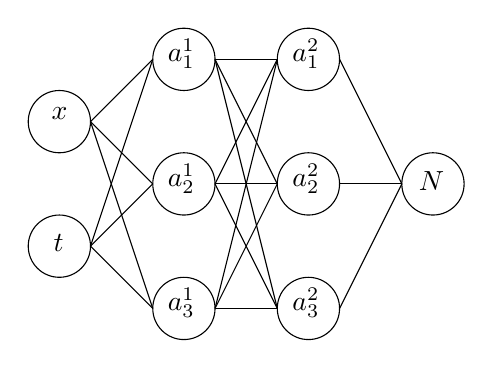
\begin{tikzpicture}[x=0.75pt,y=0.75pt,yscale=-1,xscale=1]
%uncomment if require: \path (0,695); %set diagram left start at 0, and has height of 695

%Shape: Ellipse [id:dp613538016915602] 
\draw   (80,265) .. controls (80,256.72) and (86.72,250) .. (95,250) .. controls (103.28,250) and (110,256.72) .. (110,265) .. controls (110,273.28) and (103.28,280) .. (95,280) .. controls (86.72,280) and (80,273.28) .. (80,265) -- cycle ;
%Shape: Ellipse [id:dp15712636391006307] 
\draw   (80,205) .. controls (80,196.72) and (86.72,190) .. (95,190) .. controls (103.28,190) and (110,196.72) .. (110,205) .. controls (110,213.28) and (103.28,220) .. (95,220) .. controls (86.72,220) and (80,213.28) .. (80,205) -- cycle ;
%Shape: Ellipse [id:dp8164179950038163] 
\draw   (140,175) .. controls (140,166.72) and (146.72,160) .. (155,160) .. controls (163.28,160) and (170,166.72) .. (170,175) .. controls (170,183.28) and (163.28,190) .. (155,190) .. controls (146.72,190) and (140,183.28) .. (140,175) -- cycle ;
%Shape: Ellipse [id:dp47375219812723146] 
\draw   (140,235) .. controls (140,226.72) and (146.72,220) .. (155,220) .. controls (163.28,220) and (170,226.72) .. (170,235) .. controls (170,243.28) and (163.28,250) .. (155,250) .. controls (146.72,250) and (140,243.28) .. (140,235) -- cycle ;
%Shape: Ellipse [id:dp712019427556807] 
\draw   (140,295) .. controls (140,286.72) and (146.72,280) .. (155,280) .. controls (163.28,280) and (170,286.72) .. (170,295) .. controls (170,303.28) and (163.28,310) .. (155,310) .. controls (146.72,310) and (140,303.28) .. (140,295) -- cycle ;
%Straight Lines [id:da6435868346848231] 
\draw    (110,205) -- (140,175) ;
%Straight Lines [id:da08712551076022779] 
\draw    (110,265) -- (140,235) ;
%Straight Lines [id:da18860583656122687] 
\draw    (110,265) -- (140,175) ;
%Straight Lines [id:da267566031093317] 
\draw    (110,265) -- (140,295) ;
%Straight Lines [id:da6453145574577351] 
\draw    (110,205) -- (140,295) ;
%Straight Lines [id:da9129290543985238] 
\draw    (110,205) -- (140,235) ;
%Shape: Ellipse [id:dp31900160827767665] 
\draw   (200,175) .. controls (200,166.72) and (206.72,160) .. (215,160) .. controls (223.28,160) and (230,166.72) .. (230,175) .. controls (230,183.28) and (223.28,190) .. (215,190) .. controls (206.72,190) and (200,183.28) .. (200,175) -- cycle ;
%Shape: Ellipse [id:dp21066050092203037] 
\draw   (260,235) .. controls (260,226.72) and (266.72,220) .. (275,220) .. controls (283.28,220) and (290,226.72) .. (290,235) .. controls (290,243.28) and (283.28,250) .. (275,250) .. controls (266.72,250) and (260,243.28) .. (260,235) -- cycle ;
%Shape: Ellipse [id:dp8190479437064692] 
\draw   (200,235) .. controls (200,226.72) and (206.72,220) .. (215,220) .. controls (223.28,220) and (230,226.72) .. (230,235) .. controls (230,243.28) and (223.28,250) .. (215,250) .. controls (206.72,250) and (200,243.28) .. (200,235) -- cycle ;
%Shape: Ellipse [id:dp9436580210127415] 
\draw   (200,295) .. controls (200,286.72) and (206.72,280) .. (215,280) .. controls (223.28,280) and (230,286.72) .. (230,295) .. controls (230,303.28) and (223.28,310) .. (215,310) .. controls (206.72,310) and (200,303.28) .. (200,295) -- cycle ;
%Straight Lines [id:da5770582110402913] 
\draw    (170,175) -- (200,175) ;
%Straight Lines [id:da378598346323751] 
\draw    (170,175) -- (200,235) ;
%Straight Lines [id:da045787154766960936] 
\draw    (170,175) -- (200,295) ;
%Straight Lines [id:da10461814863080832] 
\draw    (170,295) -- (200,175) ;
%Straight Lines [id:da18820240172871194] 
\draw    (170,295) -- (200,235) ;
%Straight Lines [id:da7563044436713307] 
\draw    (170,295) -- (200,295) ;
%Straight Lines [id:da9591828994155338] 
\draw    (170,235) -- (200,295) ;
%Straight Lines [id:da039530432138651816] 
\draw    (170,235) -- (200,235) ;
%Straight Lines [id:da03185694587768484] 
\draw    (170,235) -- (200,175) ;
%Straight Lines [id:da6835990243055697] 
\draw    (230,235) -- (260,235) ;
%Straight Lines [id:da4490575310089562] 
\draw    (230,295) -- (260,235) ;
%Straight Lines [id:da36571324995783205] 
\draw    (230,175) -- (260,235) ;

% Text Node
\draw (91,258) node [anchor=north west][inner sep=0.75pt]    {$t$};
% Text Node
\draw (90,197) node [anchor=north west][inner sep=0.75pt]    {$x$};
% Text Node
\draw (146,164) node [anchor=north west][inner sep=0.75pt]    {$a^{1}_{1}$};
% Text Node
\draw (146,224) node [anchor=north west][inner sep=0.75pt]    {$a^{1}_{2}$};
% Text Node
\draw (146,284) node [anchor=north west][inner sep=0.75pt]    {$a^{1}_{3}$};
% Text Node
\draw (206,164) node [anchor=north west][inner sep=0.75pt]    {$a^{2}_{1}$};
% Text Node
\draw (267,228) node [anchor=north west][inner sep=0.75pt]    {$N$};
% Text Node
\draw (206,224) node [anchor=north west][inner sep=0.75pt]    {$a^{2}_{2}$};
% Text Node
\draw (206,284) node [anchor=north west][inner sep=0.75pt]    {$a^{2}_{3}$};


\end{tikzpicture}
 
   \caption{Possible network structure of a Feed-Forward network with input $(x,t)$ and 2 hidden layers each with 3 neurons with activations denoted as $a^l_j$ and a single output $N$.}
\end{figure}


\subsection{A Nonlinear System of Ordinary Differential Equations for Finding Eigenvalues and Eigenvectors of Real Symmetric Matrices}
\noindent
For our second example, we investigate the use of neural networks for the solution of a nonlinear system of ordinary differential equations. The particular use case is the system of differential equations presented by \cite{Yi_2004} for finding the largest eigenvalue $\lambda_{1}$ and corresponding eigenvector $\pmb{v}_1$ of an $N \times N$ real and symmetric matrix $\mathbf{A}$:

\begin{equation}
\label{eq:yi_eq}
\frac{\dd \pmb{x}(t)}{\dd t} = - \pmb{x}(t) + [\pmb{x}(t)^T \pmb{x} \mathbf{A} - (1 - \pmb{x}(t)^T \pmb{x}(t)) \mathbb{I} ] \pmb{x}(t)
\end{equation}

where $\pmb{x}(t)$ is a $ 1 \times N$ column vector and $\mathbf{I}$ is an $N \times N$ identity matrix. In \cite{Yi_2004} it is shown that for any initial vector $\pmb{x}(0)$ which is not orthogonal to eigenspace of the eigenvalue $\lambda_1$, the solution $\pmb{x}(t)$ of the system \ref{eq:yi_eq} as $t$ goes to infinity converges to an eigenvector $\pmb{v}_1$ corresponding to the largest eigenvalue of $\mathbf{A}$. It is further shown in \cite{Yi_2004} that replacing $\mathbf{A}$ with $\mathbf{-A}$ in \ref{eq:yi_eq} makes the solution converge instead to an eigenvector of the smallest eigenvalue $\lambda_N$ belonging to $\mathbf{A}$, so long as the initial vector $\pmb{x}(0)$ is not orthogonal to the eigenspace of that eigenvalue $\lambda_N$. Finally, they give the following recipe for obtaining the eigenvalue from the converged eigenvector:

\begin{equation}
\label{eq:yi_eigenvalue}
\lambda = \frac{\pmb{v}^T \mathbf{A} \pmb{v}}{\pmb{v}^T \pmb{v}}
\end{equation}
which follows immediately from the definition of eigenvectors and eigenvalues.

Thus, given a real and symmetric matrix, the largest and smallest eigenvalues along with their corresponding eigenvectors can easily obtained from solving \ref{eq:yi_eq} with an appropriate initial vector $\pmb{x}(0)$. Now, in order to obtain the remaining eigenvalues and eigenvectors one could in principle apply a deflation technique, like Hotelling's or Wielandt's deflation \cite{Saad_2011} \cite{Roberts}, to the matrix $\mathbf{A}$ and repeat the process for the deflated matrix $\mathbf{A}_D$. That is, however, beyond the scope of our present work; and furthermore, non-trivial numerical issues might be expected to arise in such repeated solutions of \ref{eq:yi_eq}.

\subsubsection{Solution through the Forward-Euler Method}
\noindent
The authors of \cite{Yi_2004} presented the equation \ref{eq:yi_eq} in the context of Recurrent Neural Networks (RNN), where it describes the dynamics of a certain class of such networks. RNNs are outside our current areas of expertise; however, to the best of our knowledge, the simplest RNN that obeys the dynamics prescribed by \ref{eq:yi_eq} should be completely equivalent to the following explicit integration method (Forward-Euler):

\begin{equation}
    \label{eq:yi_euler}
    \pmb{x}(t_{i} + \Delta t) = \pmb{x}(t_i) + \frac{\dd \pmb{x}(t_i)}{\dd t}  \Delta t
\end{equation}
where $\Delta t = t_{i+1} -t_{i}$ is a suitably small time-step,  $\frac{d \pmb{x}(t_i)}{dt}$ is equation \ref{eq:yi_eq} evaluated at $t=t_i$, and the iterations are started from some initial vector $\pmb{x}(0)$.

This is, in any case, the simplest numerical integration scheme for solving equation \ref{eq:yi_eq}, and is what we will be using to compare our neural network-based solutions with.

\subsubsection{Solution through Neural Networks}
\noindent
The procedure for solving equation \ref{eq:yi_eq} with a neural network is very much the same as for the heat equation. First a trial solution satisfying the initial conditions is constructed, in this case we use:

%% TRIAL FUNCTION
\begin{equation}
    \tilde{\pmb f}(t) = \pmb x_0 e^{-t} + (1 - e^{-t}) \pmb N(t, P)
\end{equation}

Then the cost-function to be optimized is defined, in this case as:

%% COST FUNCTION
\begin{widetext}
\begin{equation}
    \mathcal C\qty[\tilde{\pmb f}(t)] = \frac{1}{M}\sum_{i}^M \qty[ 
    \dv{\tilde{\pmb f}_i(t)}{t} - \qty(- \tilde{\pmb f}_i(t) + \qty(\tilde{\pmb f}_i^T(t)\tilde{\pmb f}_i(t) \mathbf{A} + 
    \qty(1 - \tilde{\pmb f}^T_i(t) \mathbf{A} \tilde{\pmb f}_i(t)) \mathbb I) \tilde{\pmb f}_i(t))]^2
\end{equation}
\end{widetext}
Where again, this cost function is valid for a single sample $t$, and for mini-batches one would sum the cost over all the sampled $t$ and take the mean.

Finally the derivatives of the cost-function with respect to the network parameters are computed, and the network parameters are updated using Adam.

The only real change from the case of the heat equation is that the network now must produce $M$ outputs for each input $t$, as opposed to one output for each pair $x,t$ of inputs.

\begin{figure*}[h!tb]
    \center
    \subfloat[Model I evaluated on 11x11 grid]{
    \includegraphics[width=.5\columnwidth]{PDE_RELU_10_10x1000.pdf}
    }
    \subfloat[Model I evaluated on 100x100 grid]{
    \includegraphics[width=.5\columnwidth]{PDE_RELU_10_100x100.pdf}
    }
    \subfloat[Error of model I]{
    \includegraphics[width=.5\columnwidth]{PDE_RELU_10_ERR.pdf}
    }
    \\
    \subfloat[Model II evaluated on 11x11 grid]{
    \includegraphics[width=.5\columnwidth]{PDE_RELU_100_10x10.pdf}
    }
    \subfloat[Model II evaluated on 100x100 grid]{
    \includegraphics[width=.5\columnwidth]{PDE_RELU_100_100x100.pdf}
    }
    \subfloat[Error of model II]{
    \includegraphics[width=.5\columnwidth]{PDE_RELU_100_ERR.pdf}
    }
    \caption{\label{fig:ReLU composite figure}Feed-Forward Neural Networks with 4 hidden layers each consisting of 100 Neurons using the ReLU activation function trained on $11\times11$ (Model I) and $100\times100$ (Model II) equispaced points in the intervals $[x,t]\in[0,1]\times[0,1]$, where absolute error, and mean absolute error (MAE) are computed with respect to the analytic solution of the PDE on a grid of $200\times200$ equispaced points in the same interval.}
\end{figure*}

\section{Results \& Discussion}

\subsection{The Heat Equation}

% Mention network structure; describe process of implementation, experimentation etc
\noindent
We solved the heat equation (Eqn.~\ref{fig: heat eqn analytic}) in the domain $[x,y] \in [0,1]\times[0,1]$ using a Feed-Forward Neural network and an explicit Forward-Euler scheme. Both methods where then benchmarked against the analytical solution to the PDE which we derived in Section~\ref{sec:Heat equation analytical}. All the results contained in this report may also be reproduced by running the Jupyter notebooks located in our Github repository \cite{github_repo}, which also contains some additional supplementary results.

The Neural Network was implemented using the PyTorch \cite{NEURIPS2019_9015} machine learning library, chosen for its flexible interface enabling us to easily tailor our network to fit the problem at hand. When designing our model, we experimented with various network depths and layer sizes as well as activation functions, and found a reasonable balance between convergence rate and computational cost by using deep neural network with 4 hidden layers each consisting of 100 neurons. We also found good convergence with a learning weight of 0.002 and utilizing the standard set of parameters in the ADAM optimizer as proposed by its authors \textcite{kingma2017adam}. Lastly, we used an identity activation in the outer layer, as we may not in general infer about the range of a solution a priori. 

The main results of our investigations are presented in Fig.~\ref{fig:ReLU composite figure}, where we compared the output of of two identical Neural networks using the ReLU activation in the hidden layers trained on $[11\times11]$\footnote{11 being chosen instead of 10 for more symmetric plots!} and $[100\times100]$ equispaced grids for trained for $10^4$ and $10^2$ epochs respectively, with mini-batches of size $16$. The differing training time being justified by the fact that both networks will undergo approximately\footnote{Approximately because $11^2 \approx 100$} the same number of total iterations. We then computed the absolute error as well as the mean absolute error (MAE) with respect to the analytic solution on a $[200\times200]$ equispaced grid to gauge the performance of both models. We further present identical networks also trained on $[11\times11]$ equispaced grids, but instead using the Sigmoid and $\tanh$ activation functions where the evaluation and error is computed in the same way as before. The results for this is found at the end of the report in Fig.~\ref{fig:tanh sig composite figure}.

Lastly, we solved the Heat equation using the Finite-Difference scheme discussed in section~\ref{sec:finite difference theory} in the same domain for step-sizes $\Delta x = 1/10$ and $\Delta x = 1/100$ with $\Delta t$ being chosen as to satisfy the stability criterion $\Delta t / \Delta x \leq 1/2$, both the solutions and the associated errors are presented in Fig~\ref{fig:fw euler PDE error}.

\begin{figure}[h!tb]
    \center
    \subfloat[$\Delta x = 1/10,\enspace \Delta t =  1/200$]{
    \includegraphics[width=.5\columnwidth]{heat_eq_euler_10.pdf} 
    }
    \subfloat[$\Delta x = 1/100,\enspace \Delta t = 1/20000$]{
    \includegraphics[width=.5\columnwidth]{heat_eq_euler_100.pdf} 
    }
    \\
    \subfloat[$\Delta x = 1/10,\enspace \Delta t =  1/200$]{
    \includegraphics[width=.5\columnwidth]{heat_eq_euler_err_10.pdf} 
    }
    \subfloat[$\Delta x = 1/100,\enspace \Delta t = 1/20000$]{
    \includegraphics[width=.5\columnwidth]{heat_eq_euler_err_100.pdf} 
    }
    \caption{\label{fig:fw euler PDE error}Solution of the heat equation solved by finite difference (Top row) as well as the  Absolute error (Bottom row) with respect to the analytic solution for $\Delta x = 1/10$ and $\Delta x = 1/100$}
\end{figure}

In our initial experimentation with different activation functions, we found that ReLU seemed the most consistent at capturing the qualitative results of the heat equation, as observed by monitoring the evolution of the cost-functions as the networks were being trained. The full results of these models are omitted from the report, but can be found in the fully rendered Jupyter notebooks in our repo. We thus used the ReLU activation as a basis for our subsequent analysis.

We observe in Fig.~\ref{fig:ReLU composite figure} that both models seems to yield essentially the same performance, where in particular the smaller data set is able to produce similar accuracy to the much larger dataset, whilst being two orders of magnitude smaller in size. However, when compared to the solutions by Finite-Difference, the Neural network performs rather poorly in terms of accuracy. However, one thing to note in favor of the Neural network is that we are able to evaluate over the entirety of the domain $[0,1]\times[0,1]$, not just on the grid points we trained it on, but any other points in the domain. In contrast, for the solution provided by the finite difference method, we would have to utilize interpolation methods or redo the calculation with the desired points included in the computational grid. Significantly, we do not need the training points to obey the same constraints as the finite-difference method, that is; the stability criterion $\Delta t / \Delta x \leq 1/2$. That is, if we were to increase the resolution in $x$, the resolution in $t$ must be increased quadratically, blowing up if one wishes high resolution in $x$ for the finite-difference scheme. This is in stark contrast to the neural network, which can be trained on similar resolutions in both dimensions.

It should further be noted that we are not entirely confident that our network is optimized, and one may possibly with further time and tweaking obtain a neural network yielding a higher accuracy. However, given that our network has successfully reproduced the general features of the true solution, the method seems to work for solving PDEs. 

% Present the results, compare with FW euler scheme
% Intrepret the results:
% - small and large sets produce approximately the same error
% - Both are worse than FW euler scheme
% - Does not suffer from the constraints of having a stability criterion
% - May thus be useful for high-dimensional problems suffering strongly from the curse of dimensionality; as an alternative to MC methods
% - Limited time spend optimizing the problem, but showed that it is a viable way of solving PDES, further optimization/and or computation time may converge better.
% - Surprised by difference in accuracy; may imply poor modeling and/or a bug in the implementation. leaning on the  latter given the observations in the Eigenvalue problem.
% used MAE over MSE as a metric as to not be overly optimistic of the error.



\subsection{The Eigen-problem}
\noindent 
We wish to find the extrema eigenpairs of a Real, Symmetric matrix matrix by solving a set of coupled, nonlinear differential equations presented by \textcite{Yi_2004}, Eqn.~\ref{eq:yi_eq}. We prepared a random matrix by sampling a $\mathbf Q= [6\times 6]$ array of random numbers from the standard normal distribution $\mathcal N(0, 1)$ using a fixed seed ensuring that our results are reproducible. The matrix $\mathbf Q$ was then transformed to a real, symmetric matrix $\mathbf A$ by
\begin{equation}
    \mathbf A = \mathbf Q^T + \mathbf Q
\end{equation}
%  MENTION HOW LONG THE NETWORKS ARE TRAINED, SAME AS PREVIOUSLY
Following our work on the heat equation, we used a similar approach by solving the differential equations using a Neural Network as well as an explicit Forward-Euler scheme, where the latter was used to gauge how well the network is able to reproduce the dynamics of the system. The eigenpairs produced by the network were benchmarked against the eigh method in Numpy, which calls on numerically robust methods in LAPACK. We again wished to infer about the way in which the NN solution is affected by sample sizes, and thus trained two identical neural networks on the interval $t = [0,3]$ using 30 and 300 data points. Where the appropriate interval was determined by observing whether the explicit scheme had converged. 
\vspace{5mm}
\begin{table}
    \center
    \caption{\label{tab:eigenvecs}Maximal eigenpairs predicted with the 30pt ($N_{30}$) and 300pt ($N_{300}$) models}
   \begin{tabular}{|l |r | r @{\hspace{1em}} r @{\hspace{1em}} r @{\hspace{1em}} r @{\hspace{1em}} r @{\hspace{1em}} r|}
    \hline
              & $\lambda_{max}$ & $x_1$ & $x_2$ & $x_3$ & $x_4$ & $x_5$ & $x_6$ \\ \hline 
    $N_{30}$  & 3.689 & 0.535 & -0.007 & -0.281 & 0.696 & 0.223 & -0.318 \\
    $N_{300}$ & 3.707 & 0.551 & -0.019 & -0.306 & 0.676 & 0.224 & -0.308 \\
    Numpy     & 3.722 & 0.578 & -0.021 & -0.337 & 0.627 & 0.239 & -0.318 \\
    \hline
    \end{tabular} 
\end{table}
The predicted eigenpairs are shown in Table~\ref{tab:eigenvecs} for both the models, along with the eigenpairs produced by Numpy. We further present the full dynamics of the differential equations in Fig.~\ref{fig:eigenvector}. From this, we also computed the inner products between the eigenvector produced by Numpy and the eigenvectors produced by our neural networks, which yielded $\langle \pmb x_{np}, \pmb x_{30}\rangle = 0.995$ and $\langle \pmb x_{np}, \pmb x_{300}\rangle = 0.998$ for the 30 and 300 point neural networks respectively, where we note that the eigenvectors are normalized.

As our first and most striking observation, we see in Fig.~\ref{fig:eigenvector} that the network based solution to a large degree, but not fully, mimics the solution from the Forward-Euler scheme. Interestingly, for the present computational domains, the results seems to be largely independent of the number of points used in the training set given a comparable amount of training in both cases. Whilst we have not been able to fully reproduce the dynamics suggested by the Forward-Euler, the qualitative reproduction of their character by the models is such as to suggest that given more training and tweaking of the networks one may obtain a more accurate reproduction.

Secondly, we remark that the eigenpairs computed by both networks provide reasonable estimates of the ground truth. There is however a problem with relying solely on the solutions to the differential equations produced by the neural network to infer about the eigenpairs, namely due to the difficulty in determining whether the end of the time domain corresponds to a steady state solution. If one wishes to compute the eigenpairs, one needs to pick a time domain such that the true solutions have reached a steady state and converged to the components of the eigenvector, however, we do not in general have a method for picking a suitable time domain without prior knowledge of the dynamics. To illustrate this point; if we did not know the dynamics of the solutions a priori, the choice between time domains of $[0,3]$ and for example $[0,0.5]$ is completely arbitrary, where in the latter case one could never hope to produce the eigenvectors, as seen in Fig.~\ref{fig:eigenvector}. At the other extreme, experiments with overly large time-domains seemed to significantly degrade the convergence of the network-based solution to the Forward-Euler solution. Thus, we are not convinced that using neural networks to solve the differential equations (Eqn.~\ref{eq:yi_eq}) is a very useful way of computing eigenpairs.

We also computed the minimal eigenpairs in a completely identical manner by substituting $\mathbf A$ with $- \mathbf A$, given that the results are rather similar to the ones we have already looked at, we will not discuss there further and simply refer the reader to the Jupyter notebook for the results.


% Mention network structure; describe process of implementation, experimentation etc
% - Manages to qualitatively reproduce the main features of the dynamics of the highly non-linear system of coupled DE's 
% - Eigenvalue & Eigenvalues are approximated to a pretty good degree of accuracy, but pales in comparrison to numpy
% - More training & model optimization is likely required to achieve better accuracy; but serves as a good proof of concept
% - Attempted to find eigenvalues by longer durations; however eigenvalues where rather poor. Thus implying that proper sampling of the early system may be an important factor in the final prediction of the network. This makes the network a rather poor candidate for finding eigenvalus, given that it would require a priori knowledge of the appropriate timespan to solve the sytstem for, which for anything past a toy problem is not feasable. Given that you may as well use a standard DE solver in that case. We did in fact encounter this exact problem, where the positive eigenvalues where converged, but the negative ones were not. 
% When we went on find the smalles eigenvalue; we found that the explicit scheme had not yet converged to a steady state, meaning that no matter what, our eigenvalues would not be correct.

\begin{figure}[h!tb]
   \center
   \subfloat[30 Points]{\includegraphics[width=.5\columnwidth]{eigenvec_dynamics.pdf}}
   \subfloat[300 Points]{\includegraphics[width=.5\columnwidth]{eigenvec_dynamics_100.pdf}}
   \caption{\label{fig:eigenvector} Dynamics of the eigenvector components of the largest eigenvalue of the matrix $A$ modeled by Neural networks (Solid lines) trained on 30 and 300 datapoints as well as the same dynamics solved using a Forward Euler method (dotted lines) where Numpy eigenvector components is indicated by the semi-transparent dashed lines.}
\end{figure}


\section{Conclusion}

We have successfully applied neural networks to the solution of both partial differential equations and systems of nonlinear ordinary differential equations. We find that our neural network-based models reasonably reproduce the true solutions; getting the right qualitative behavior, but achieving mediocre accuracy as compared to more standard methods. The main issue is that the training in our current implementation appears to stall/plateau once a certain degree of accuracy has been reached.

For most domains we tried, the network-based solutions seemed largely independent of number of training points; so long as the total number of training iterations was similar, the results were similar. This indicates that a further increase in the number of training points will not help the accuracy, conversely fairly few training points are required to obtain a decent approximation, at least for the cases we have considered. This could be described as a blessed curse, one of the more obvious ways for improving the accuracy looks dishearteningly ineffective. On the other hand, as mentioned previously, a somewhat reasonable solution can be computed on a quite limited set of data-points, and, crucially, be directly evaluated on any point in the trained domain. That represents one of the clear advantages of neural network-based solutions as contrasted with traditional finite-difference schemes, which require either interpolation or recomputation on a finer or shifted grid. 

An observation we made, but have not pursued in any level of detail, is that the extent of the domain we solve for seemed to have a sizable impact on the convergence of the solutions. Extending the training domain far into the steady-state region for the eigenpair-example lead to qualitatively worse reproduction of the dynamics. One important limitation of our investigation is that the points were either randomly sampled from uniform distribution, or taken as an equidistant grid. Conceivably it might have lead to better accuracy if more training points were clustered around rapidly varying parts of the solutions.

Other possible approaches for improving the accuracy of the network solutions include even further training, tweaking of the optimization-procedure/learning rate, testing different network architectures or even experimenting with different forms of the trial solutions (as they are not unique). Particularly, the fact that we see very small changes to the solution with further training indicate a need for more aggresive learning rates; or possibly some error in our implementation. Though the qualitative reproduction of the true solutions gives us confidence in the correctness of our results, it is not definite proof that the implementation is free of bugs.

For the considered example cases, the solutions based on neural networks were not at all competitive with those from standard methods. Especially for the  eigenpair-porblem it seems like using neural networks to solve the differential equation is a bad approach if the goal is the eigenpairs themselves. However, we want to reiterate that \cite{Yi_2004} do not suggest using neural networks to solve the differential equation \ref{eq:yi_eq}, they propose using a RNN whose dynamics obey that equation for finding eigenpairs. That might very well be a promising approach for matrices whose dimensions make standard numerical linear-algebra-methods appear unappetizing.

While the cases we have considered do not look too favorable for the network-based solutions, we would like to point out that our experiments have been with fairly low-dimensional problems. The benefit of neural networks might first kick in at higher dimensions. To wit, it is quite easy to setup trial functions for arbitrarily large dimensions, while the corresponding finite-difference schemes become more and more burdensome to both implement and compute. Other numerical integration methods like finite-element methods (FEM) also face serious difficulties when the dimensionality of the problem increases; if the neural networks-based approaches can be made more accurate, we believe there to be a large niche of multidimensional problems where they may find themselves superior to traditional methods.

In summary, we have shown some potential for neural networks to solve both partial differential equations and systems of nonlinear differential equations. We find that accuracy is an issue, but recognize that there are many avenues to investigate in search of improving that issue. As the potential benefits of neural networks applied to high-dimensional problems are significant, we deem it a fruitful area for further study.




%Okay, but not great accuracy
%Gets the qualitative behaviour mostly right
%Difficult to increase accuracy
%%Trial functions are far from unique, possible to use better ones
%%For most domains we tried, largely independent on number of training points; so long as the total number of training iterations was similar. Limitation that the points were either randomly sampled from uniform distribution, or taken as an equidistant grid.
%Seems, but not tested extensively, sensitive to the problems domain, indicates that it requires far more training when the solutions vary between staying stable for a long stretch and changing rapidly
% Ideas for improving accuracy: nonuniform sampling of points, much more patience with the training, additional tweaking of the optimizer and/or the learning rate, more experimentation with different trial functions.
% Particularly, small changes to the solution over large training periods indicate need for more aggresive learning rates and/or error in our implementation. Though the qualitative reproduction gives us confidence in the correctness of our results, it is not definite proof.

%% But there are advantages.
% - The true benefit of the may become apparent by looking at higher dimensional problems
% - "trivial" to implement; no need to discretize, setting up finite-diff schemes is tedious for higher dimensions
% The full "landscape" may be reproduced well by small, incomplete datasets. Also observed in terrain data previously => Neural networks may be suitable for high dimensional problems with limited sampling. More sampling of rapidly changing regions could easily be done to conceivably improve the solution. Not completely trivial to locally refine a finite-difference grid for high-dimensionalities.
% In summary, very interesting  for continued study. Accuracy is an issue, but there are many avenues to investigate in search of improvement.

\onecolumngrid
\bibliography{bibfile}
\twocolumngrid

\end{document}